\documentclass[tikz,border=4pt]{standalone}
% Estilo común de los diagramas de bloques (se usa con \input en cada standalone)
\usepackage[defaultsans,scale=0.92]{lato}
\usepackage{libertinust1math}
\usepackage{xcolor,amsmath}
\usepackage{tikz}
\usetikzlibrary{positioning,arrows.meta,calc,shapes.geometric}
\usepackage{../../notacion}
\definecolor{ctrlazul}{HTML}{1E5AA8}\definecolor{ctrlnoche}{HTML}{14213D}
\definecolor{ctrlcoral}{HTML}{D1495B}\definecolor{ctrlverde}{HTML}{2A9D8F}
\definecolor{ctrlambar}{HTML}{E09F3E}\definecolor{ctrlgris}{HTML}{5C677D}
\definecolor{ctrlvioleta}{HTML}{6C4AB6}\definecolor{ctrlteal}{HTML}{0F7173}
\tikzset{
  >={Stealth[length=2.4mm]}, every node/.style={font=\small},
  bloque/.style={draw=ctrlnoche,fill=ctrlazul!7,thick,rounded corners=1.5pt,minimum height=9mm,minimum width=13mm,inner sep=4pt},
  suma/.style={draw=ctrlnoche,thick,circle,inner sep=0pt,minimum size=6mm},
  senal/.style={->,thick,draw=ctrlnoche},
  rot/.style={font=\footnotesize,text=ctrlgris},
}

\begin{document}
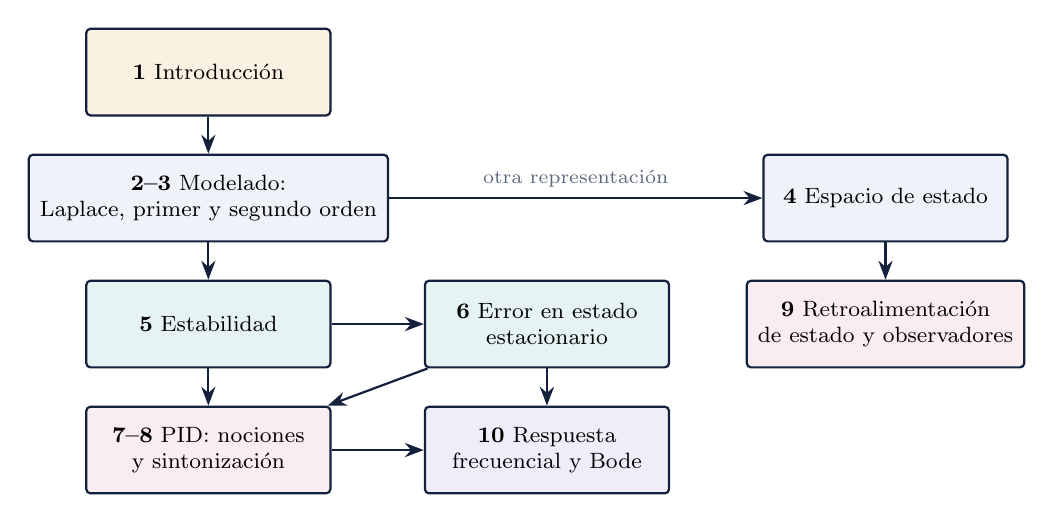
\begin{tikzpicture}[c/.style={bloque,minimum width=31mm,minimum height=11mm,font=\footnotesize,align=center},
  e/.style={font=\scriptsize,text=ctrlgris,align=center}]
  \node[c,fill=ctrlambar!15] (c1) at (0,0) {\textbf{1} Introducción};
  \node[c] (c2) at (0,-1.6) {\textbf{2--3} Modelado:\\Laplace, primer y segundo orden};
  \node[c] (c4) at (8.6,-1.6) {\textbf{4} Espacio de estado};
  \node[c,fill=ctrlverde!12] (c5) at (0,-3.2) {\textbf{5} Estabilidad};
  \node[c,fill=ctrlverde!12] (c6) at (4.3,-3.2) {\textbf{6} Error en estado\\estacionario};
  \node[c,fill=ctrlcoral!10] (c9) at (8.6,-3.2) {\textbf{9} Retroalimentación\\de estado y observadores};
  \node[c,fill=ctrlcoral!10] (c7) at (0,-4.8) {\textbf{7--8} PID: nociones\\y sintonización};
  \node[c,fill=ctrlvioleta!10] (c10) at (4.3,-4.8) {\textbf{10} Respuesta\\frecuencial y Bode};
  \draw[senal] (c1)--(c2); \draw[senal] (c2)--node[above,e]{otra representación}(c4); \draw[senal] (c2)--(c5);
  \draw[senal] (c5)--(c6); \draw[senal] (c5)--(c7); \draw[senal] (c6)--(c7);
  \draw[senal] (c4)--(c9); \draw[senal] (c6)--(c10); \draw[senal] (c7)--(c10);
\end{tikzpicture}
\end{document}
